\documentclass{beamer}
\usepackage[T1]{fontenc}
\usepackage[utf8]{inputenc}

% Enables Portuguese Brasil
\usepackage[portuguese]{babel}

% Enables code listing
\usepackage{listings}

%Enables the use of greek letter without a math context
\usepackage{textgreek}

\usepackage{ragged2e}

% Enables math chars
\usepackage{amsmath}

% Enables section slides
\AtBeginSection[]{
	\begin{frame}
	\vfill
	\centering
	\begin{beamercolorbox}[sep=8pt,center,shadow=true,rounded=true]{title}
		\usebeamerfont{title}\insertsectionhead\par
	\end{beamercolorbox}
	\vfill
	\end{frame}
}


%Information to be included in the title page:
\title{Monografia apresentada para cumprimento da disciplina de estudos especiais}
\author{André Furlan - ensismoebius@gmail.com}
\institute{Universidade Estadual Paulista Júlio de Mesquita Filho}
\date{2019}
\logo{
\includegraphics[height=1cm]{unesp.png}}
\usetheme{Madrid}

\begin{document}
	
	%Start frame
	\frame{\titlepage}
	
	%2
	\begin{frame}
		\frametitle{Estrutura da apresentação}
		\begin{itemize}
			\item Revisão de conceitos utilizados.
			\item Trabalhos correlatos.
			\item Contextualização.
		\end{itemize}
	\end{frame}

	\section{Revisão de conceitos utilizados}

	\begin{frame}
		\frametitle{Engenharia paraconsistente de características}
		\only<1>{
			\framesubtitle{Os vetores de características proporcionam uma boa separação interclasses?}
			\begin{columns}
			\column{0.7\textwidth}				
			\begin{figure}
				\centering
				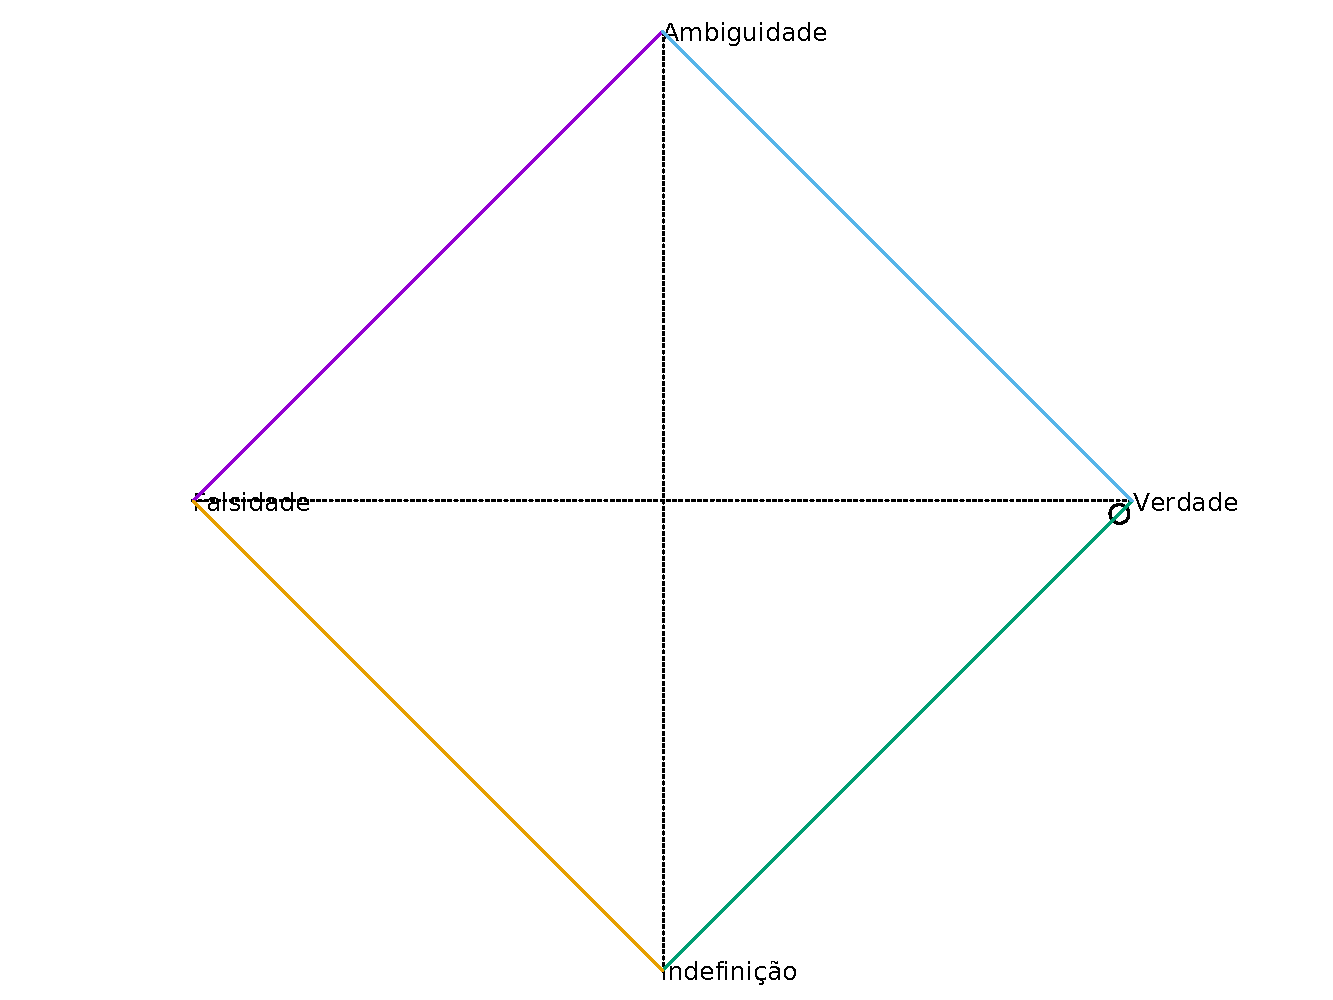
\includegraphics[width=0.8\linewidth]{images/paraconsistentPlane}
				\label{fig:paraconsistentplane}
				\caption{Plano paraconsistente}
			\end{figure}
			\column{0.3\textwidth}
			\begin{itemize}
				\item Verdade:\\
				 $\alpha = 1$ e $\beta = 0$.
				\item Ambiguidade:\\
				 $\alpha = 1$ e $\beta = 1$.
				\item Falsidade:\\
				 $\alpha = 0$ e $\beta = 1$.
				\item Indefinição:\\
				 $\alpha = 0$ e $\beta = 0$.
			\end{itemize}
		\end{columns}
		}
		\only<2>{
			\framesubtitle{Cálculo de $\alpha$}
			\begin{figure}
				\centering
				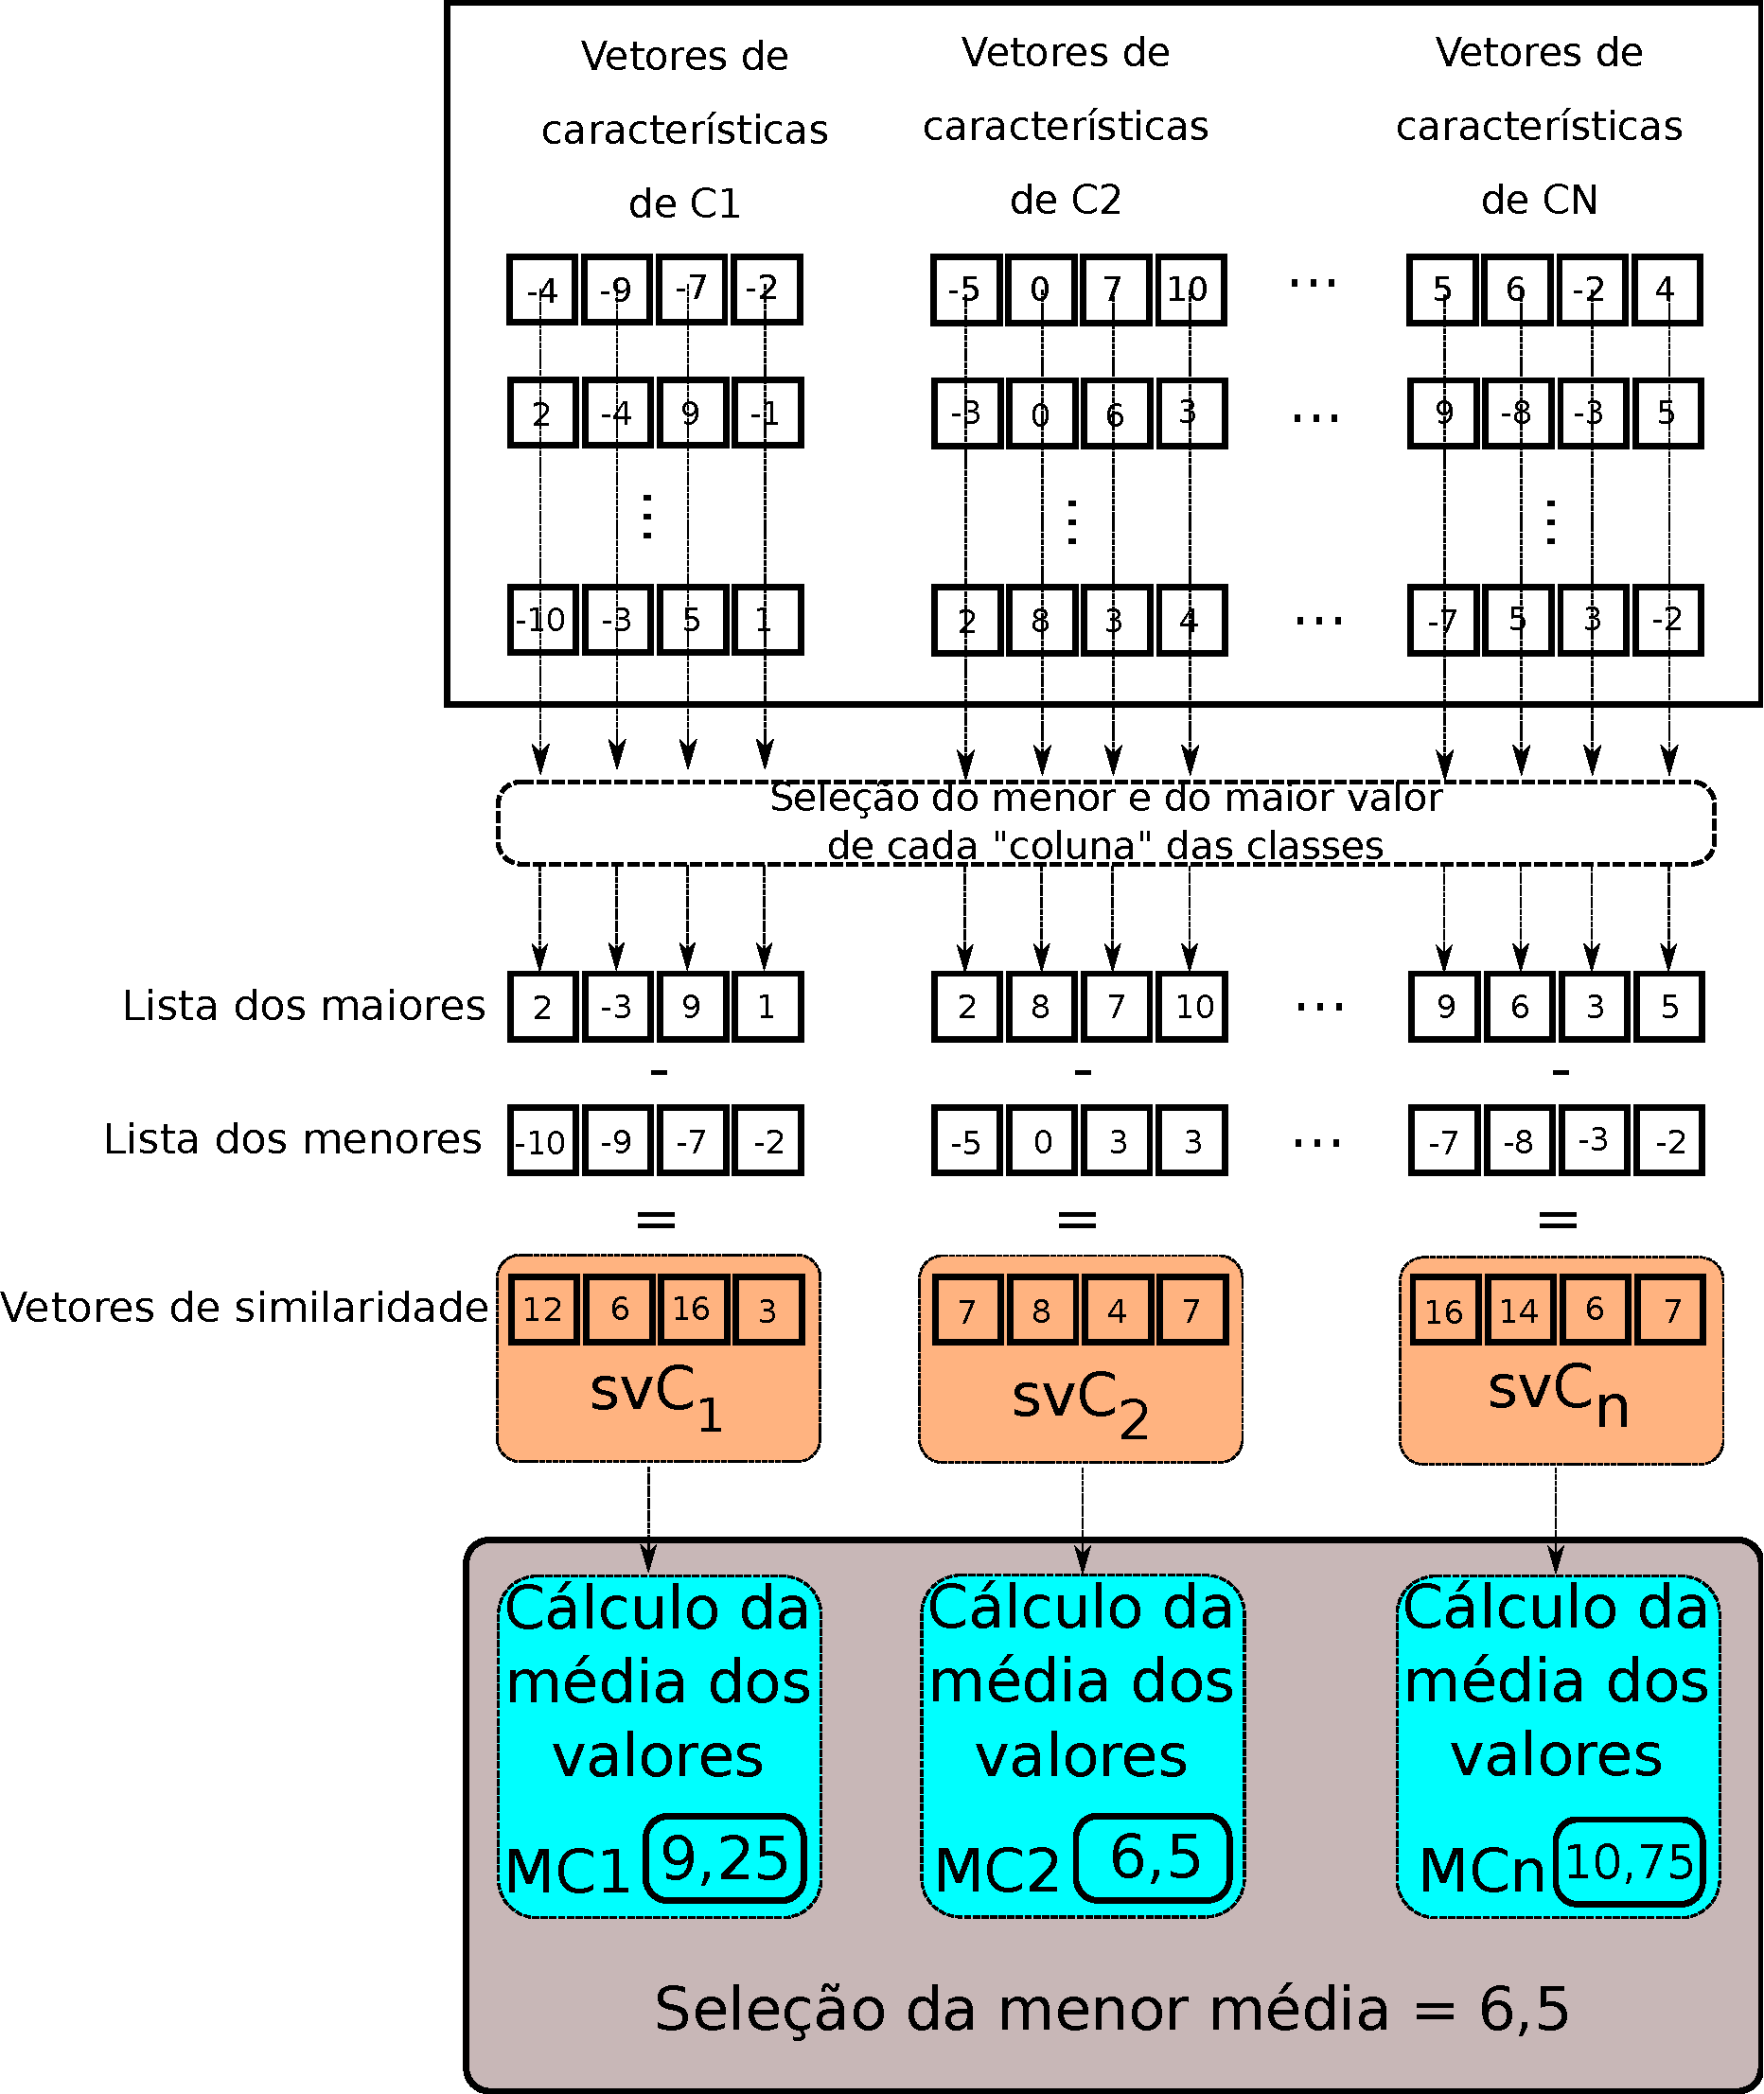
\includegraphics[height=0.82\textheight]{images/calculoAlpha}
				\label{fig:calculoalpha}
			\end{figure}
		}
		\only<3>{
			\framesubtitle{Cálculo de $\beta$}
				\begin{figure}
				\centering
				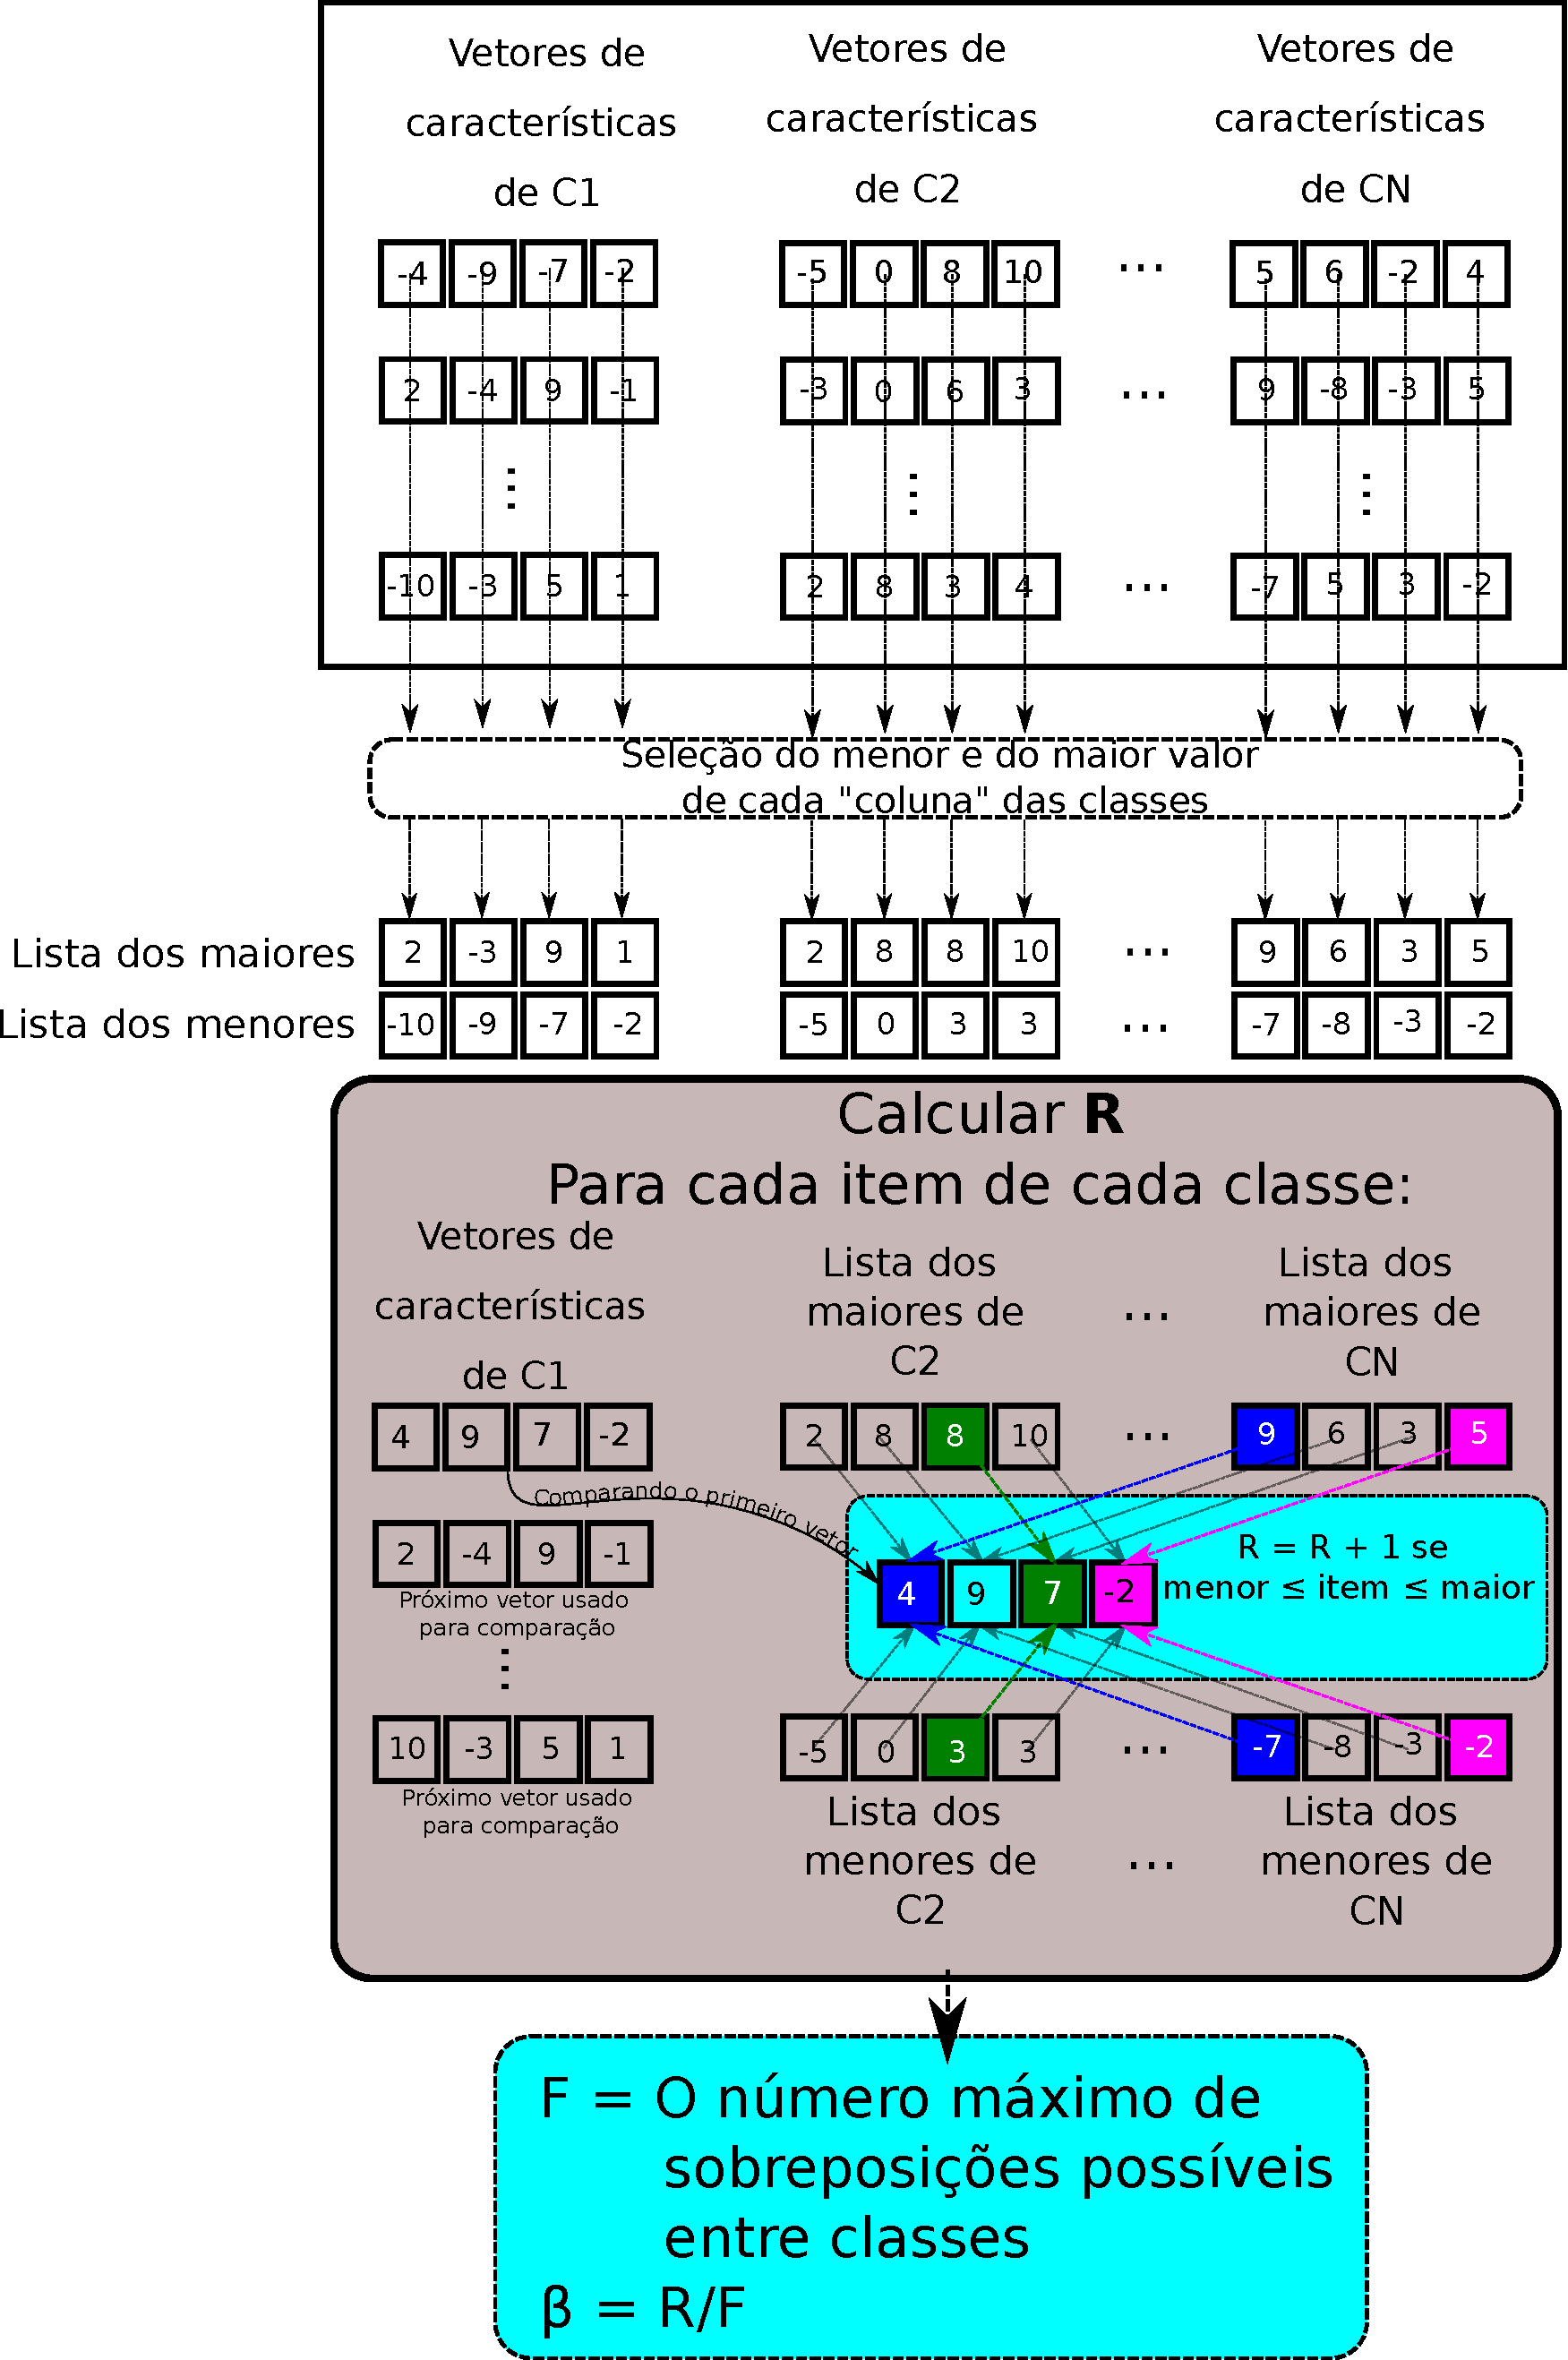
\includegraphics[height=0.82\textheight]{images/betaCalculation.pdf}
				\label{fig:calculobeta}
			\end{figure}
		}
		\only<4>{
			\framesubtitle{Graus de certeza e contradição}
			\begin{itemize}
				\item Grau de certeza $\rightarrow G_1=\alpha-\beta $.
				\item Grau de contradição $\rightarrow G_2=\alpha+\beta-1 $.				
			\end{itemize}
			Onde: $-1 \leqslant G_1 \leqslant 1$ e  $-1 \leqslant G_2 \leqslant 1\qquad$.\\
			Seja $P=(G_1,G_2)$
			\begin{itemize}
				\item (-1,0) $\rightarrow$ Falsidade;
				\item (1,0) $\rightarrow$ Verdade;
				\item (0,-1) $\rightarrow$ Indefinição;
				\item (0,1) $\rightarrow$ Ambiguidade.
			\end{itemize}
		}
		\only<5>{
			\framesubtitle{Distancias no plano paraconsistente}
			As distâncias$(D)$ do ponto $P=(G_1,G_2)$ dos limites supracitados. Tal cálculo pode ser feito da seguinte forma:
			\begin{equation*}
			D_{-1,0}=\sqrt{(G_1+1)^2+(G_2)^2}\qquad,
			\end{equation*}
			\begin{equation*}
			D_{1,0}=\sqrt{(G_1-1)^2+(G_2)^2}\qquad,
			\end{equation*}
			\begin{equation*}
			D_{0,-1}=\sqrt{(G_1)^2+(G_2+1)^2}\qquad,		
			\end{equation*}
			\begin{equation*}
			D_{0,1}=\sqrt{(G_1)^2+(G_2-1)^2}\qquad,
			\end{equation*}
		}
	\end{frame}
	
	\begin{frame}
		\frametitle{Filtros digitais \textit{wavelet}}
		\only<1>{
			\framesubtitle{Propriedades}
			\begin{itemize}
				\item Tamanho de janelas variável.
				\item Análise multiresolução.
				\item Análise detalhada em altas e baixas frequências.
			\end{itemize}
		}
		\only<2>{
			\framesubtitle{Restrição de escopo}
			\begin{itemize}
				\item Apenas transformadas diretas.
				\item Não haverá reconstrução do sinal.
				\item Construção de vetores de características.
				\item Domínio discreto.
			\end{itemize}
		}

		\only<3>{
			\framesubtitle{\textit{Wavelets} de Daubechies}
			\begin{columns}
			\column{0.5\textwidth}
				\begin{figure}
					\centering
					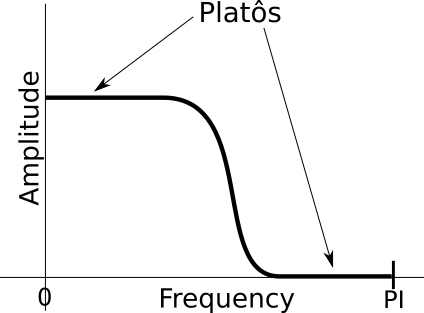
\includegraphics[width=\linewidth]{images/daubechies}
					\caption{platôs maximamente planos em um filtro digital}
					\label{fig:daubechies}
				\end{figure}
			\column{0.5\textwidth}
				\begin{figure}
					\centering
					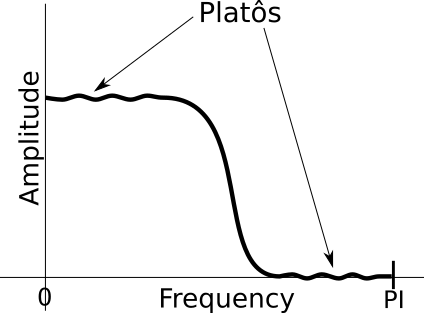
\includegraphics[width=\linewidth]{images/noMaximallyFlat}
					\caption{platôs não maximamente planos de um filtro digital}
					\label{fig:nomaximallyflat}
				\end{figure}
			\end{columns}
		}
		\only<4>{
			\framesubtitle{Algoritmo de Malat}
			\begin{itemize}
				\item \textit{Wavelet} Haar: $h[\cdot] = [\frac{1}{\sqrt{2}}, \frac{1}{\sqrt{2}}]$.
				\item Par ortogonal: $g[\cdot] = [\frac{1}{\sqrt{2}}, \frac{-1}{\sqrt{2}}]$.
				\item sinal: $s[\cdot] = [1,2,3,4]$.
			\end{itemize}
			
			\begin{equation*}
			\begin{pmatrix}
			\frac{1}{\sqrt{2}}, \frac{1}{\sqrt{2}}, 0, 0\\
			\frac{1}{\sqrt{2}}, \frac{-1}{\sqrt{2}}, 0, 0\\
			0, 0, \frac{1}{\sqrt{2}}, \frac{1}{\sqrt{2}}\\
			0, 0, \frac{1}{\sqrt{2}}, \frac{1}{\sqrt{2}}\\
			\end{pmatrix} 
			\cdot
			\begin{pmatrix}
			1\\
			2\\
			3\\
			4\\
			\end{pmatrix} 
			=
			\begin{pmatrix}
			\frac{3}{\sqrt{2}}\\
			\frac{-1}{\sqrt{2}}\\
			\frac{7}{\sqrt{2}}\\
			\frac{-1}{\sqrt{2}}\\
			\end{pmatrix}
			\Rightarrow \Big[
			\frac{3}{\sqrt{2}},
			\frac{7}{\sqrt{2}},
			\frac{-1}{\sqrt{2}},
			\frac{-1}{\sqrt{2}}
			\Big]\qquad.
			\end{equation*}
		}

	\end{frame}
	\begin{frame}
		\frametitle{Amostragem, quantização e o formato do arquivo \textit{Wave}}
		\begin{columns}
		\column{0.6\textwidth}
			\begin{figure}
				\centering
				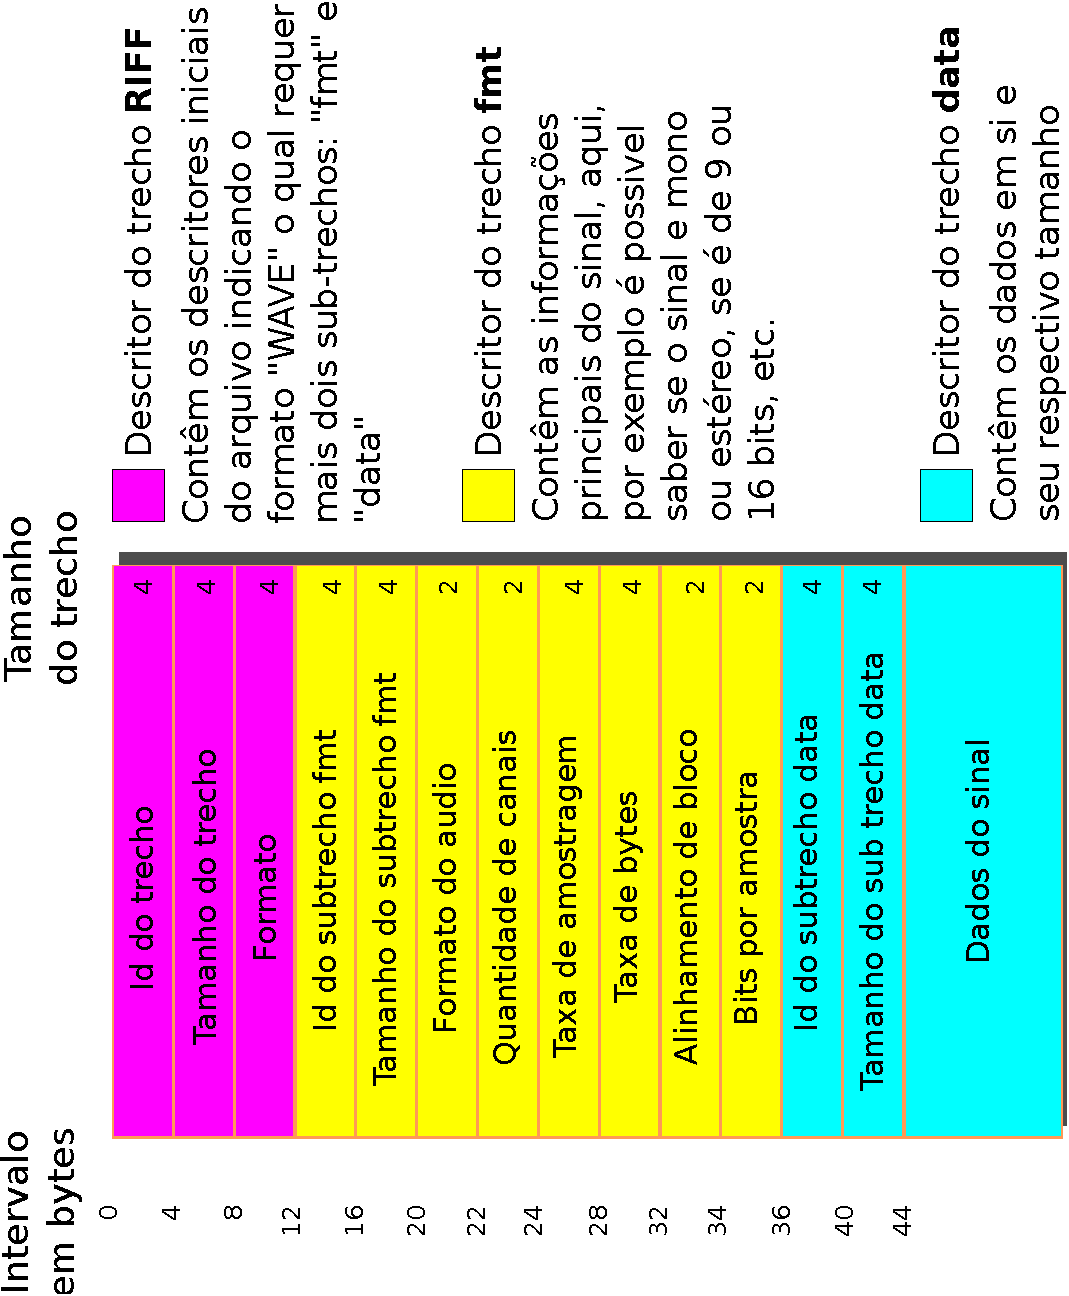
\includegraphics[width=0.88\linewidth, angle=-90]{images/wavePcmStructure.pdf}
				\label{fig:wavePcmStructure}
			\end{figure}
		\column{0.4\textwidth}
			\begin{itemize}
				\item Formato \textit{wave}.
				\item \textit{Pulse-code modulation} (PCM).
				\item Taxa de amostragem de 44100hz.
				\item Resolução de 16bits
			\end{itemize}
		\end{columns}
	\end{frame}

	\begin{frame}
		\frametitle{Caracterização dos processos de produção da voz humana}
		\only<1>{
			\framesubtitle{Áreas de estudo}
			\begin{itemize}
				\item Fisiológica ou fonética articulatória.
				\item Acústica ou fonética acústica.
				\item Perceptual.
			\end{itemize}
			\textbf{Foco apenas na acústica}
		}
		\only<2>{
			\framesubtitle{Vozeada versus não-vozeada}
			\begin{itemize}
				\item Vozeada: Pregas vocais.
				\item Não vozeada: Sem pregas vocais.
			\end{itemize}
		}
		\only<3>{
			\framesubtitle{Frequência fundamental da voz}
			\begin{itemize}
				\item Conhecida como $F_0$.
				\item Componente periódico resultante da vibração das pregas vocais.
			\end{itemize}
		}
		\only<4>{
			\framesubtitle{Formantes}
			\begin{itemize}
				\item $F_1 \rightarrow$ amplificação  sonora  na  cavidade  oral  posterior,  posição  da  língua  no  plano  vertical.
				\item $F_2 \rightarrow$ cavidade  oral  anterior,  posição  da  língua  no  plano  horizontal.
				\item $F_3 \rightarrow$ cavidades  à  frente  e  atrás  do  ápice  da  língua.
				\item $F_4 \rightarrow$ formato da laringe e da  faringe.
			\end{itemize}
		}
	\end{frame}

	\section{Trabalhos correlatos}

	\begin{frame}[allowframebreaks]
		\frametitle{Trabalhos correlatos}
		\begin{itemize}
			\item \cite{Ren2019}: Energia e outras várias características do espectro do sinal, SVM.
			\item \cite{DiqunYan2019} \textit{Modelo oculto de Markov} (HMM); \textit{Wavelets}, SVM.
			\item \cite{7802552} \textit{Wavelets}, coeficientes cepstrais (SCCs), Modelos de mistura Gaussiana (GMM).
			\item \cite{alluri2019replay} \textit{"Zero time windowing"}(ZTW), análise cepstral do espectro GMM.
			\item \cite{8725688} Coeficientes cepstrais, GMM.
			\item \cite{Hanilci2018} Predição linear, coeficientes cepstrais, GMM.
			\item \cite{ISI:000473343500086} ``Texturas de voz'', padrões binários locais (LBP) e seus respectivos histogramas, SVM.
			\item \cite{TODISCO2017516} \textit{Transformada de constante Q} (CQT), Processamento cepstral, fusão de dois classificadores GMM, sendo que um deles usa \textit{coeficientes cepstrais de frequência MEL}(MFCC) e o outro usa características CFCC-IF \cite{Patel2015}; STC \cite{7472724}; SJTU \cite{korshunov2016overview}.
			\item \cite{ISI:000490497200068} Partes não vozeadas da fala, três GMMs.
			\item \cite{ISI:000465363900136} amplitude instantânea vinda de flutuações de energia, GMM.
			\item \cite{ISI:000465363900139} Diferenças entre bandas de frequências específicas, \textit{predição linear em domínio de frequência}(FDLP), GMMs.
			\item \cite{Suthokumar2018} \textit{Modulation  spectral  centroid  frequency}, \textit{long term spectral average}, GMM.
			\item \cite{ISI:000458728700054} Envelopamento das amplitudes e das frequências instantâneas em cada banda estreita filtrada, GMM.
			\item \cite{ISI:000392503100008} \textit{Gammatone frequency cepstral coefficients}(MGFCC), GMM.
			\item \cite{8396208} \textit{Hashing} sensível a locus(LSH), MFCC e LSH, \\
			tabela \textit{hash}. 
		\end{itemize}
	\end{frame}

	\section{Contextualização}

	\begin{frame}
		\frametitle{Contextualização}
		\begin{itemize}
			\item Características mais disjuntas possíveis para de ``locutor autêntico'' e ``ataque de \textit{voice spoofing}''.
			\item \textit{Wavelet}: Boa resolução em relação às dimensões de tempo e frequência.
			\item Análise paraconsistente de acordo com o trabalho \cite{8588433}.
		\end{itemize}
	\end{frame}

	\begin{frame}[allowframebreaks]
		\frametitle{Referências}
		\bibliography{bibliography.bib}
		\bibliographystyle{alpha}
	\end{frame}
	
\end{document}